%! suppress = MissingImport
The 74LS20 ``chip'' is an integrated circuit (IC) that holds two 4-input NAND gates.
It is in a \textit{dual inline package} (DIP), and solderless breadboards are designed for the DIP form factor to straddle the breadboard's center divider.
A notch on the left side of the DIP helps us orient the IC; the pins are numbered counter-clockwise from the lower-left to the upper-left (Figure~\ref{fig:nand-annotated}).
The relationship between the 74LS20's pins and the NAND gates' inputs and outputs is shown in Figure~\ref{fig:nand-pinout}.

Figure~\ref{fig:nand-diagram} shows the wiring to install the 74LS20.

\begin{figure}
    \centering
    \subfloat[Pin numbers for the 74LS20.]{
        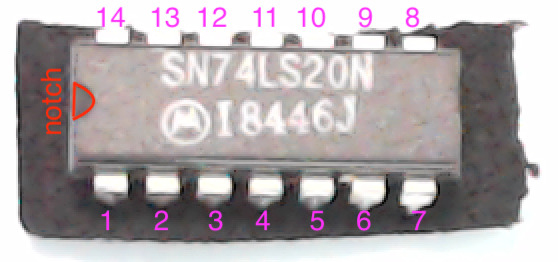
\includegraphics[width=6cm]{direct/nand/nand-annotated}
        \label{fig:nand-annotated}
    }
    \hfil
    \subfloat[Connection diagram showing the 74LS20's pinout.]{
        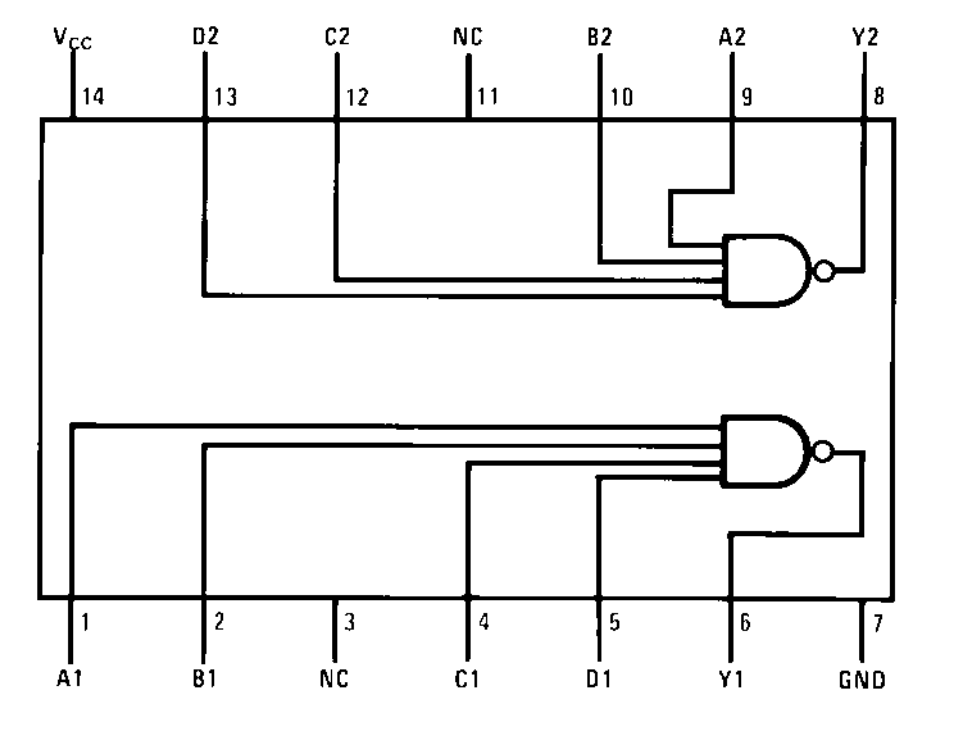
\includegraphics[width=6cm]{direct/nand/nand-pinout}
        \label{fig:nand-pinout}
    }
    \caption{Pin information for the 74LS20.}
\end{figure}

\begin{figure}
    \centering
    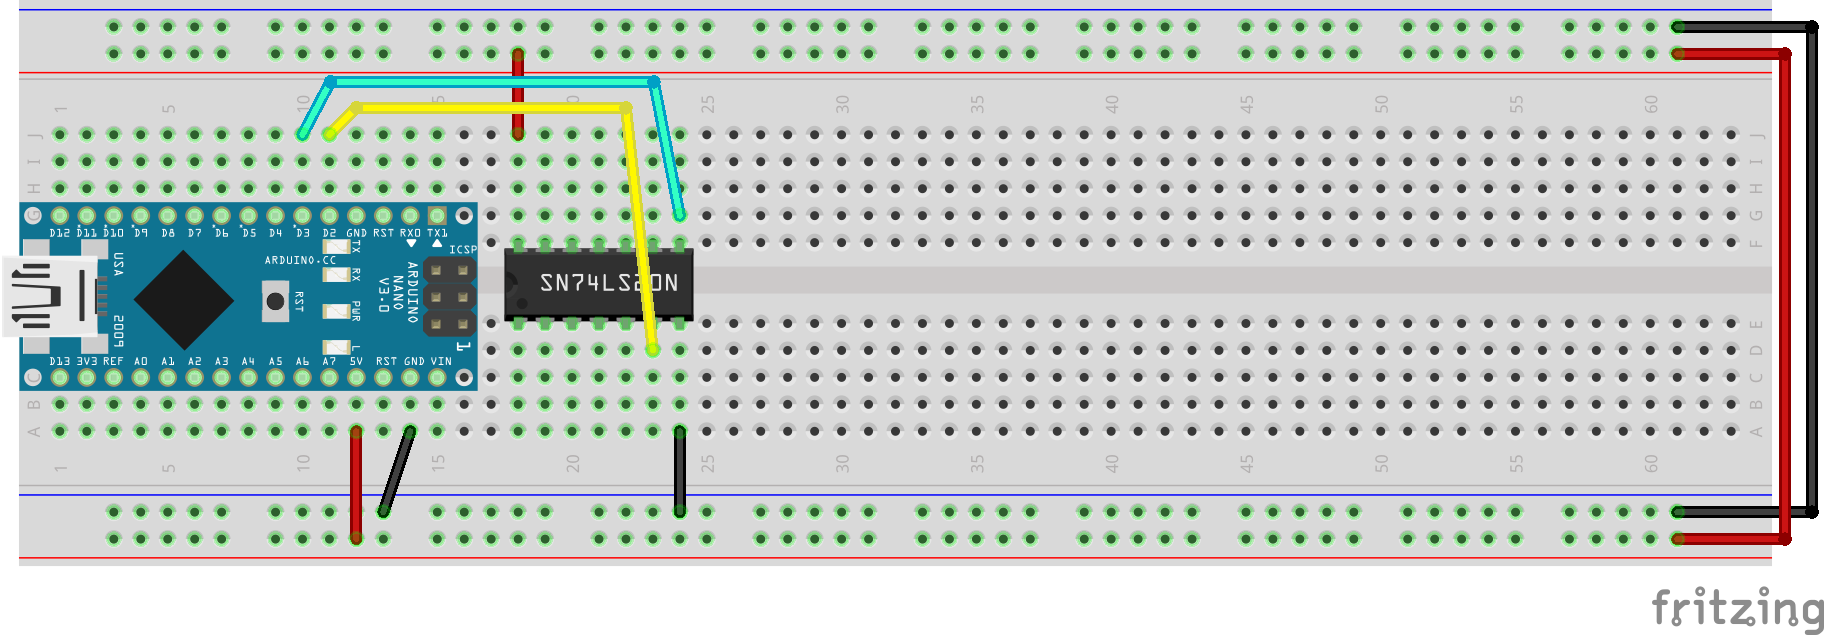
\includegraphics[width=0.9\textwidth]{fritzing_diagrams/nand}
    \caption{Diagram of the 74LS20's installation. \label{fig:nand-diagram}}
\end{figure}

\disconnect\

\prepunch{\nandupperrow\ and \nandlowerrow}

Remove the anti-static foam from the 74LS20's pins.
As described in the \href{https://learn.adafruit.com/breadboards-for-beginners/breadboard-usage}{guide at adafruit.com}, gently press the 74LS20's pins against a tabletop until they're approximately square to the IC's case.
With its notch to the left, place the 74LS20 on the breadboard straddling the center divider on rows 18--24.
Double-check that the 74LS20's pins 1--7 are on contact points \nandlowerrow\ and that pins 8--14 are on contact points \nandupperrow\ (Figure~\ref{fig:nand-ready} shows that the IC's pins are not splayed outside the contact points nor are folded under the IC's case).
Gently press on the 74LS20 to insert the pins into the contact points, using a slight rocking motion if necessary.
As shown in Figure~\ref{fig:nand-inserted}, the IC is fully inserted when its case is flush with the breadboard.

\begin{figure}
    \centering
    \subfloat[Integrated circuit ready to be inserted.]{
        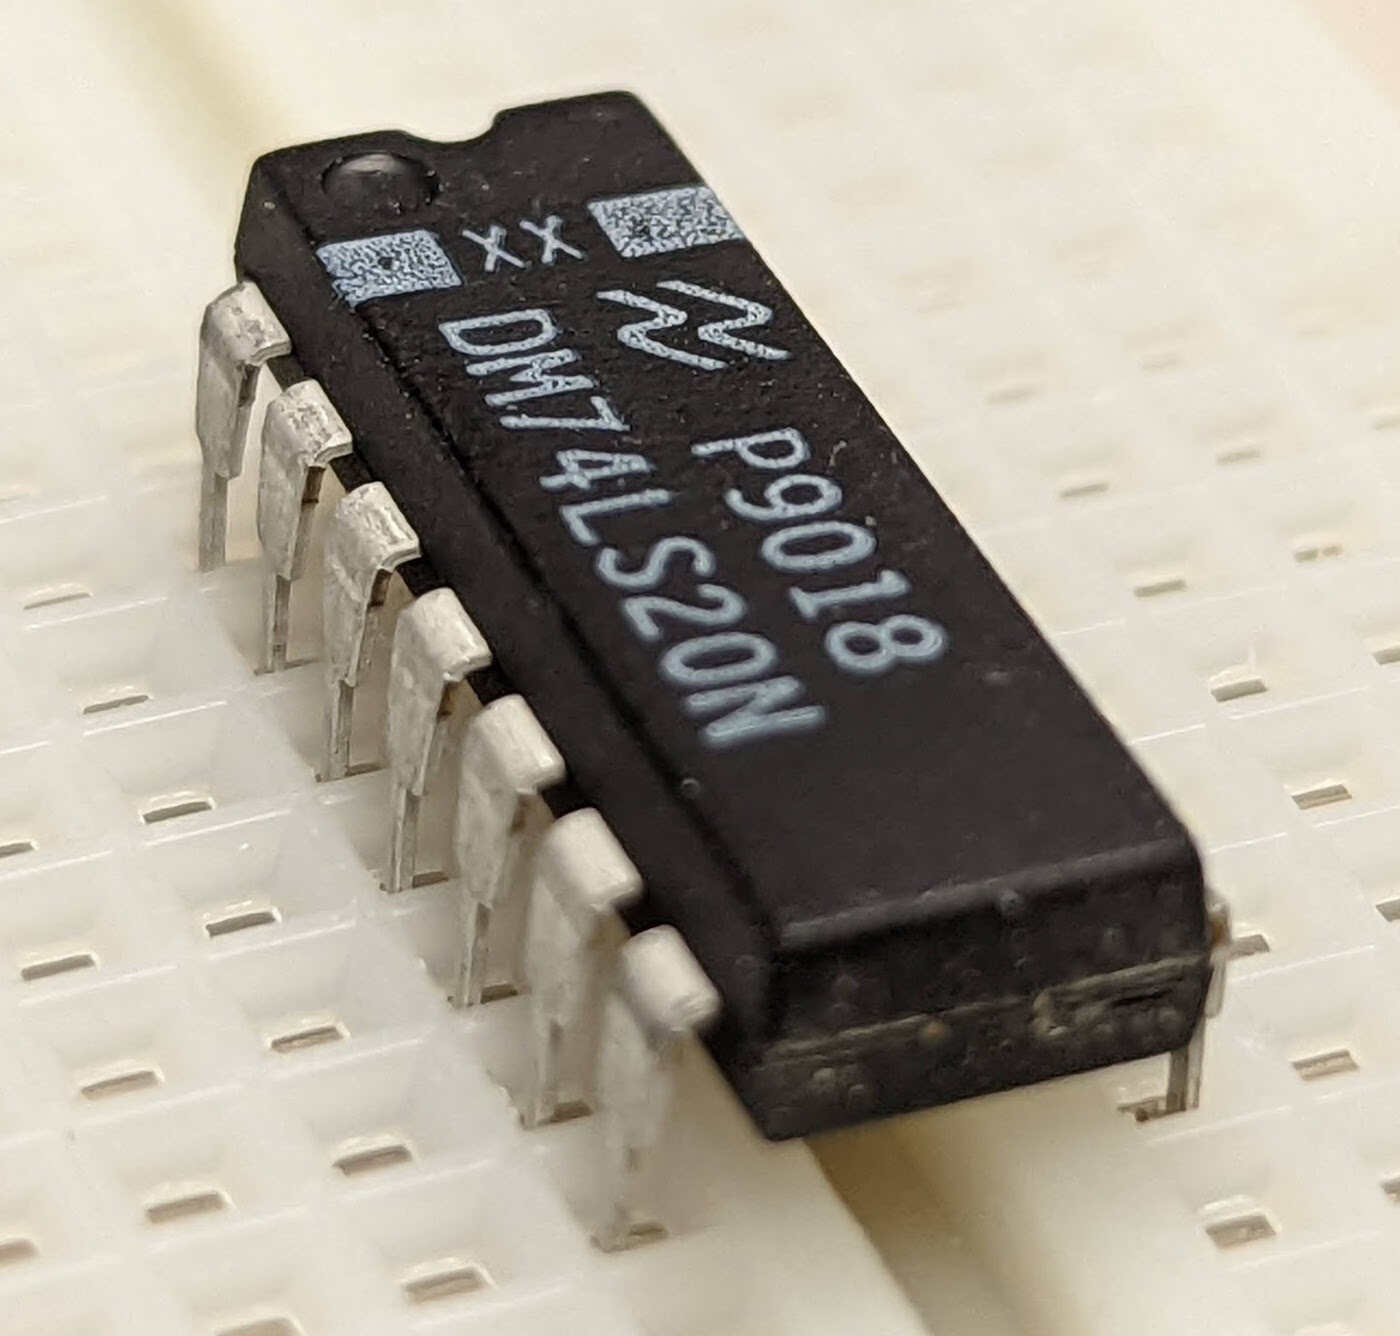
\includegraphics[height=4cm]{direct/nand/nand-ready-to-insert}
        \label{fig:nand-ready}
    }
    \hfil
    \subfloat[Integrated circuit fully inserted.]{
        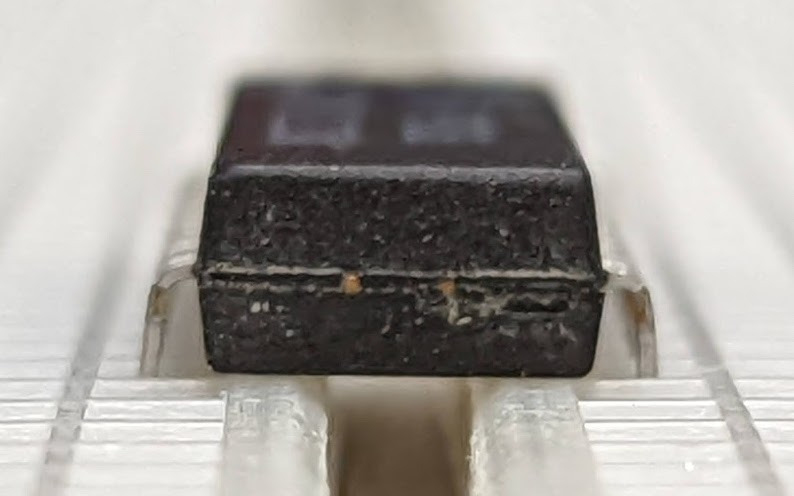
\includegraphics[height=4cm]{direct/nand/nand-fully-inserted}
        \label{fig:nand-inserted}
    }
    \caption{Inserting the 74LS20.}
\end{figure}

Peel one wire from the \rainbow;
use this wire to connect contact point \nandvcc\ (electrically connected to the 74LS20's $\mathtt{V_{CC}}$, pin 14) to the upper \power.
Peel off another wire from the \rainbow;
use this wire to connect contact point \nandground\ (electrically connected to the 74LS20's \texttt{GND}, pin 7) to the contact point \mculowergroundcontactpoint\ (electrically connected to one of the \developmentboard's \texttt{GND} pins).
See Figure~\ref{fig:nand-power}.

Peel four more wires from the \rainbow.
Use two wires to connect contact points \nandupperc\ and \nandupperd\ to the upper \power.
Use another wire to connect contact point \nanduppery\ (electrically connected to the 74LS20's \texttt{Y2}, pin 8) to contact point \mcubuttonnandpoint\ (electrically connected to the \developmentboard's \mcubuttonnand\ pin).
These three wires configured the 74LS20's upper 4-input NAND gate to act as a 2-input NAND gate;
you will provide the inputs in Section~\ref{subsec:pushbuttons}.
Use the fourth wire to connect contact point \nandlowery\ (electrically connected to the 74LS20's \texttt{Y1}, pin 6) to contact point \mcukeypadnandpoint\ (electrically connected to the \developmentboard's \mcukeypadnand\ pin);
you will  provide the inputs for the lower 4-input NAND gate in Section~\ref{sec:keypad}.
See Figure~\ref{fig:nand-outputs}.

\begin{figure}
    \centering
    \subfloat[The 74LS20 connected to power and ground.]{
        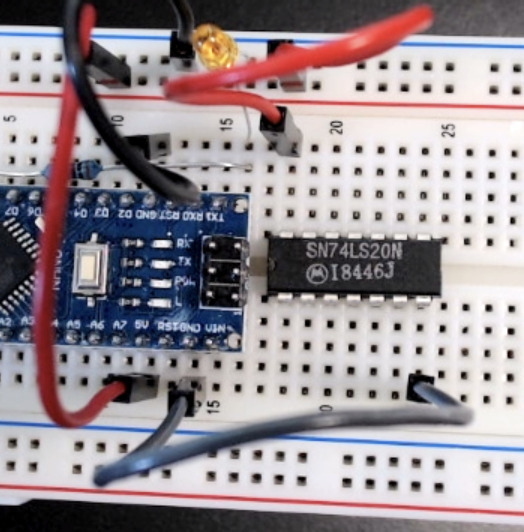
\includegraphics[width=.4\textwidth]{direct/nand/nand-power}
        \label{fig:nand-power}
    }
    \hfil
    \subfloat[The 74LS20's outputs connected to the \developmentboard.]{
        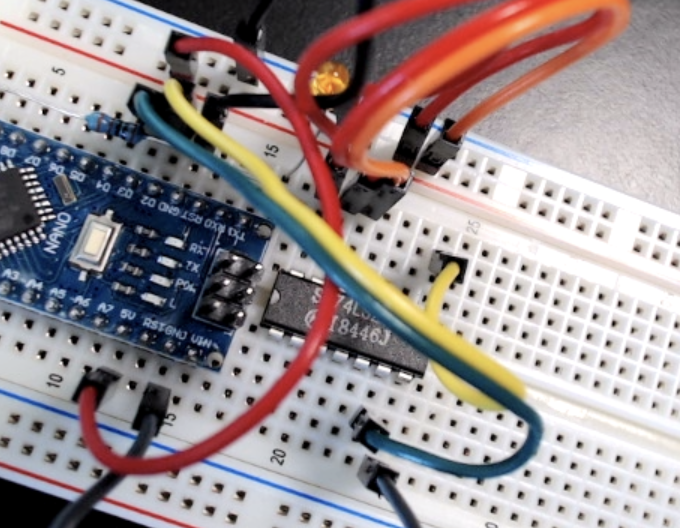
\includegraphics[width=.5\textwidth]{direct/nand/nand-outputs}
        \label{fig:nand-outputs}
    }
    \caption{Wiring the 74LS20.}
\end{figure}

When you have finished wiring the 74LS20, there should be the electrical connections described in Table~\ref{tab:nand}.

\begin{table}
    \begin{center}\begin{tabular}{||c|c|c||} \hline\hline
    74LS20 Pin  & \developmentboard\ pin    & Pulled High/Low \\ \hline
    6           & \texttt{D3}   & \\
    7           &               & Pulled Low \\
    8           & \texttt{D2}   & \\
    12          &               & Pulled High \\
    13          &               & Pulled High \\
    14          &               & Pulled High \\ \hline\hline
    \end{tabular}\end{center}
    \caption{Initial Electrical Connections for NAND Gates.\label{tab:nand}}
\end{table}

\checkpoint{inserted and wired the 74LS20}
